\section{Problem Formulation}
\label{sec:notation}

% In this section, we provide background on uncertain graphs, privacy attack and justify our choice of utility loss metric. 
% On this basis, we present our formulation of the uncertain graph anonymization problem. 
In this section, we present background on uncertain graphs, show possible privacy attacks, and formulate the privacy notion for releasing privacy-preserving uncertain graphs. We also justify our choice of utility loss metric. Finally, we present our formulation of the uncertain graph anonymization problem. 

\subsection{Uncertain Graph}
An uncertain graph $\mathcal{G}=(V,E,\mathit{p})$, is defined over a set of nodes $V$, a set of edges $E$, and a set of probabilities $\mathit{p}$ of edge existence. Following the literature~\cite{Potamias_K_2010,Zhao_Detecting_2014,Colbourn_Colbourn_1987}, we assume the possible-worlds semantics, and we consider the edge probabilities independent \footnote{We leave the conditional probability model as a future extension.}. An uncertain graph $\mathcal{G}=(V,E,\mathit{p})$ essentially represents a probability distribution over all of the certain graphs $G$ in the forms of which the uncertain graph may actually exist. 
The probability of observing any possible world $G_i=(V,E_{G_i})$ is    
\begin{equation*}
    Pr[G_i]=\prod_{e \in E_{G_i}} {\mathit{p}(e)} \prod_{e \in E \setminus E_{G_i}} 1-\mathit{p}(e)
\end{equation*}
\subsection{Privacy Attack}
\label{sec:AMPC}
\begin{figure}[!htb]
    \subfigure[Social Trust Network]{\label{fig:socialNetwork}
      \begin{minipage}[l]{0.46\columnwidth}
        \centering
        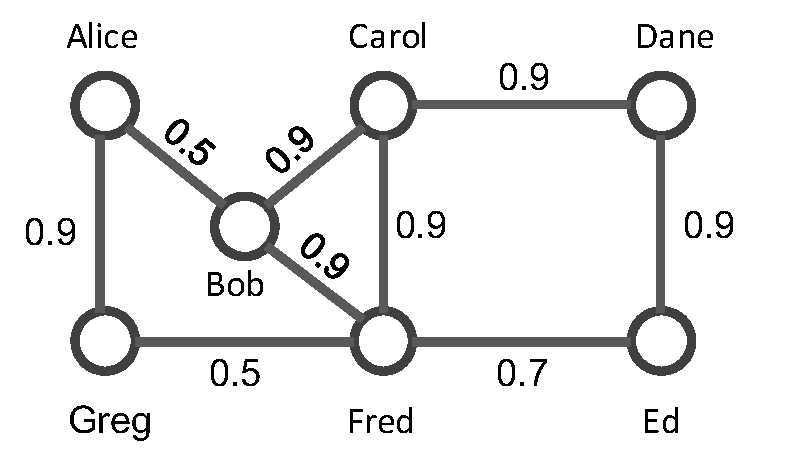
\includegraphics[height=2.7cm]{ill/example_source.pdf}
      \end{minipage}
      }
    \subfigure[The naive anonymization]{\label{fig:b2bNetwork}
      \begin{minipage}[l]{0.46\columnwidth}
        \centering
        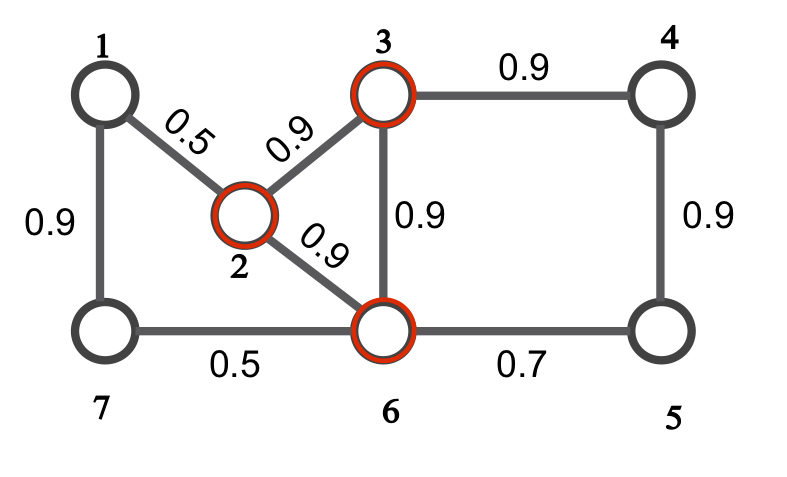
\includegraphics[height=2.7cm]{ill/example_output.jpg}
      \end{minipage}
      }
    \vspace{-4pt}
    \caption{The structural re-identification issue.}
    \label{fig:privacyAttack}
\end{figure} 
Apparently, simply removing the identities of the nodes before publishing the uncertain graph does not guarantee privacy.  The structure of the uncertain graph itself, and in its basic form the degree of the nodes, can be revealing the identities of individuals. 
In practice, the adversary may have access to external information about the entities in the graphs. This information may be obtained by the adversary's malicious actions. 

\textbf{Example.} For the uncertain graph in Figure~\ref{fig:privacyAttack}, the adversary might know that ``\emph{Fred has \textbf{three or more} trust neighbors}''. Such information allows the adversary to narrow down the set of candidates in the sanitized graphs.  The statement partially re-identify Fred as $\lbrace 2,3,6 \rbrace$ with different \textbf{probabilities} respectively. 
Different to the deterministic scenario, such posterior probabilities significantly vary over candidate nodes $\lbrace 2,3,6 \rbrace$ where $P(\text{Fred}|2) \ll P(\text{Fred}|6) \ll P(\text{Fred}|2)$ as $P(\text{Fred}|2)=0.5*0.9*0.9=0.405$ and $P(\text{Freq}|2)=0.9*0.9*0.9=0.729$ and $P(\text{Freq}|6)=0.468$. 


As ever illustrated, nodes in uncertain graphs are vulnerable to the re-identification risk. Such Entity Re-identification (ER) can lead to additional disclosures. In this work, we focus on the ER attack as it is one of the most serious privacy problems. 
\subsection{Privacy Notion}
\label{sec:privacyNotion}
In this work, we adopt $(k,\epsilon)$-obf, a variant of the well-known $k-$anonymity as the privacy notion for privacy-preserving uncertain graph releasing. 
It was proposed by Boldi {\etal} in ~\cite{Boldi_Injecting_2012}, where $k \ge 1$ is a desired level of obfuscation and $\epsilon \ge 0$ is a tolerance parameter. 

\textsc{Obfuscation Parameter}~~
Similar to $k$-candidate anonymity, 
$k-$obf requires blending every entity with other fuzzy matching entities. 
While, $k$-anonymity requires that each entity is identical with at least k-1 other entities. 
Bonchi{\etal}~\cite{Bonchi_Identity_2014} observed that $k$-anonymity does not measure the amount of uncertainty correctly that the adversary has regarding the correct identification of the target individual. 

$k$-obf generalizes the candidate anonymity concept to the probabilistic scenario by the use of entropy. 
For a given node $v$ in the real network, it quantifies the level of obfuscation that is provided for $v$ by the perturbed graphs as the entropy of $\lbrace Pr(v|u) : u \in V_{\hat{G}}  \rbrace$, where $Pr(v|u)$ stands for the posterior belief probability that $u$ is the image of the target node $v$. 

% It lower bounds the entropy of the distribution by $\log_{2}k$.
Though it is initially used to measure the anonymity provided by an uncertain graph to the deterministic graph, the stochastic nature makes it a good fit in the uncertain scenario. 

\textsc{Tolerance parameter}~~As for the tolerance parameter $\epsilon$, it serves for the following purpose. There might be extreme unique nodes, e.g., Trump in a Twitter network, whose obfuscation is almost impossible. Thus, Boldi {\etal}~\cite{Boldi_Injecting_2012} introduce a tolerance parameter $\epsilon$, which allows skipping up to $\epsilon * |V|$ nodes and makes the privacy notion more practical. 
% The formal definition is,
% \theoremstyle{definition}
% \begin{definition}
%     \textbf{\boldmath{$(k,\epsilon)$}-obf \cite{Boldi_Injecting_2012}}
%     Let $P$ be a vertex property (i.e., vertex degree in our work), $k \geq 1$ be a desired level of anonymity, and $\epsilon >0 $ be a tolerance parameter. 
%     An sanitized uncertain graph $\tilde{\mathcal{G}}$ is said to $k$-obfuscate a given vertex $v \in \mathcal{G}$ w.r.t $P$ if the entropy $H()$ of the distribution $Y_{P(v)}$ over the nodes 
%     of $\tilde{\mathcal{G}}$ is greater than or equals to $\log_{2}{k}$:
%     \begin{equation*}
%         H(Y_{P(v)}) \geq \log_{2}{k}.
%     \label{obfCon}
%     \end{equation*}
% The uncertain graph $\tilde{\mathcal{G}}$
% is $(k,\epsilon)$-obf w.r.t property $P$ 
% if it $k$-obfuscates at least $(1-\epsilon)|V|$ nodes in $\mathcal{G}$. 
% \label{def:obf}
% \end{definition} 
\subsection{Utility Loss: Reliability Discrepancy}

In the context of deterministic graphs, connectivity discrepancy is widely used to measure the structural distortion for the following reasons. 
First, the connectivity model is known to yield a better graph representation than the degree sequence model.
What's more, connectivity plays a vital role in various graph mining tasks such as nearest neighbor locating, decomposition and graph clustering. 
\begin{figure}[!htb]
  \centering
  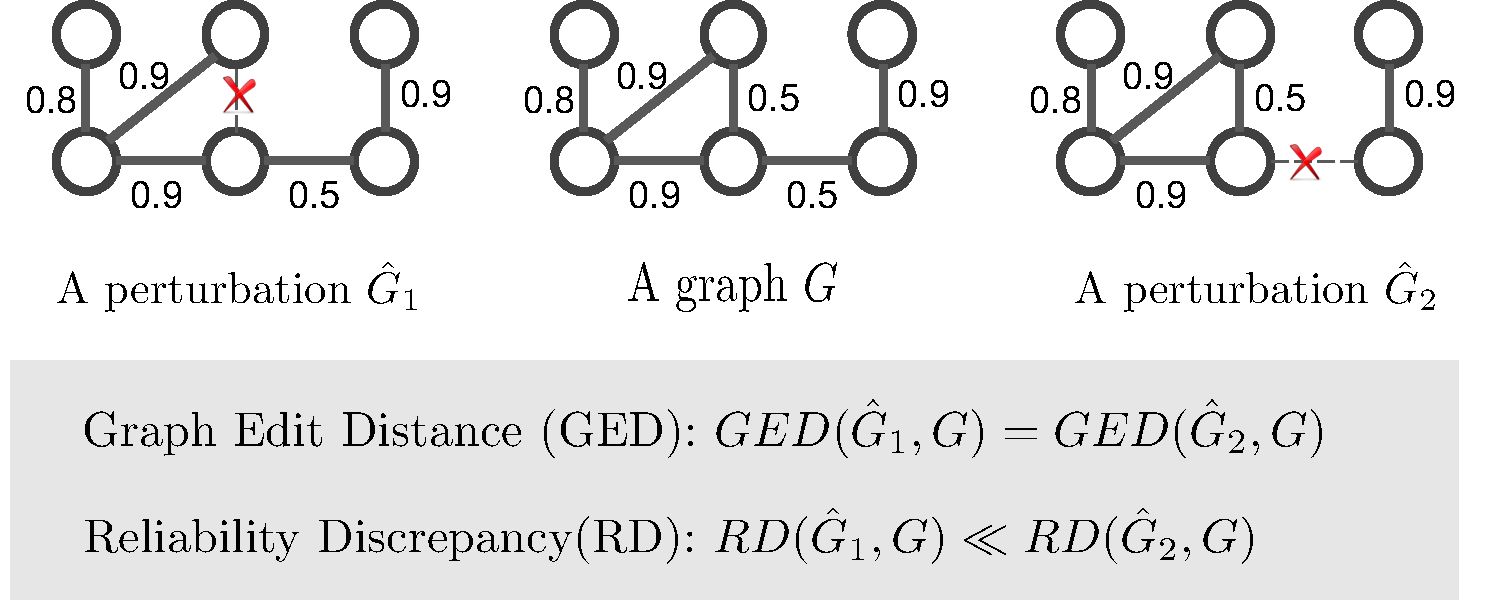
\includegraphics[height=3.3cm]{ill/UL.pdf}
  \vspace{-4pt}
  \caption{Comparison of utility loss metrics.}
  \label{fig:utility_loss}
\end{figure} 

While, the concept of reliability generalizes the connectivity concept in the uncertain scenario. 
It captures the probability that two given nodes are reachable over all possible worlds, as shown in Def~\ref{d:reliability}. 
Analogous to the deterministic case, we use reliability discrepancy as the utility-loss metric for utility safeguard, as outlined in Def~\ref{d:RD}. 
\begin{definition}
    \textbf{Two-Terminal Reliability~\cite{Colbourn_Colbourn_1987}}~~Given an uncertain graph $\mathcal{G}$, and two distinct nodes $u$ and $v$ in the graph, the reliability of $(u,v)$ is defined as:
        \begin{equation*}
                R_{u,v}(\mathcal{G})= \sum_{G \in W(\mathcal{G})} \mathcal{I}_{G}(u,v) ~ Pr[G] 
        \end{equation*}
    where Pr[G] is the probability of observing $G$ as one possible world of G, and $\mathcal{I}_{G}(u,v)$ is 1 iff $u$ and $v$ are contained in a connected component in $G$, and 0 otherwise.   
    \label{d:reliability}
\end{definition}

\theoremstyle{definition}
\begin{definition}
    \textbf{Reliability Discrepancy (RD)}
    The reliability difference between a sanitized output $\tilde{\mathcal{G}}$ and the original input $\mathcal{G}$, 
    denoted as $\Delta(\tilde{\mathcal{G}})$, 
    is defined as the sum of the two-terminal reliability discrepancy over all node pairs $(u,v) \in V_\mathcal{G}$.
    \begin{equation*}
        \Delta(\tilde{\mathcal{G}})=\sum_{(u,v) \in V_\mathcal{G} }|R_{u,v}(\mathcal{G})-R_{u,v}(\tilde{\mathcal{G}})|
    \end{equation*}
    \label{d:RD}
\end{definition}

\subsection{Problem Statement} 
% \vspace{-5pt}
\begin{problem}
     Given an uncertain graph $\mathcal{G}$ and desired anonymization parameters $k$ and $\epsilon$, 
     the objective is to find a  $(k,\epsilon)$-obf uncertain graph $\tilde{\mathcal{G}}$
     with the minimal utility loss,
     \begin{equation*}
             \begin{aligned}
                 & \argmin_{\tilde{
                \mathcal{G}}} & & \Delta(\tilde{\mathcal{G}}) \\
                &  \text{Subject to} & &\tilde{\mathcal{G}} \text{~is~} (k,\epsilon)-obf
            \end{aligned}
     \end{equation*}
     \label{prob:unobf}
\end{problem}
% add one paragraph to ....